%%%%%%%%%%%%%%%%%%%%%%%%%%%%%%%%%%%%%%%%%%%%%%%%%%%%%%%%%%%%%%%%%%%%%%%%%%%
%% This file is part of the book
%%
%% Algorithmic Graph Theory
%% http://code.google.com/p/graph-theory-algorithms-book/
%%
%% Copyright (C) 2009--2011 Minh Van Nguyen <nguyenminh2@gmail.com>
%%
%% See the file COPYING for copying conditions.
%%%%%%%%%%%%%%%%%%%%%%%%%%%%%%%%%%%%%%%%%%%%%%%%%%%%%%%%%%%%%%%%%%%%%%%%%%%

\documentclass{article}

\usepackage{subfigure}
\usepackage{tikz}
\usepackage{tkz-berge}  %% for drawing combinatorial graphs
\usetikzlibrary{external}
\tikzexternalize{Franklin-graph}

\begin{document}

\begin{figure}
\subfigure[]{
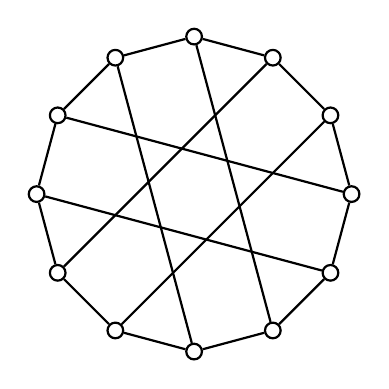
\begin{tikzpicture}
[lineDecorate/.style={-,thick},%
  nodeDecorate/.style={shape=circle,inner sep=2pt,draw,thick},%
  scale=2]
%% nodes or vertices
\foreach \nodename/\x/\y in {
  0/1/0, 1/0.866/0.5, 2/0.5/0.866, 3/0/1, 4/-0.5/0.866,
  5/-0.866/0.5, 6/-1/0, 7/-0.866/-0.5, 8/-0.5/-0.866,
  9/0/-1, 10/0.5/-0.866, 11/0.866/-0.5}
{
  \node (\nodename) at (\x,\y) [nodeDecorate] {};
}
%% edges or lines
\path
\foreach \startnode/\endnode in {
  0/1, 0/5, 0/11, 1/2, 1/8, 2/3, 2/7, 3/4, 3/10, 4/5, 4/9, 5/6, 6/7,
  6/11, 7/8, 8/9, 9/10, 10/11}
{
  (\startnode) edge[lineDecorate] node {} (\endnode)
};
\end{tikzpicture}
}
%%
%%
\qquad
\subfigure[]{
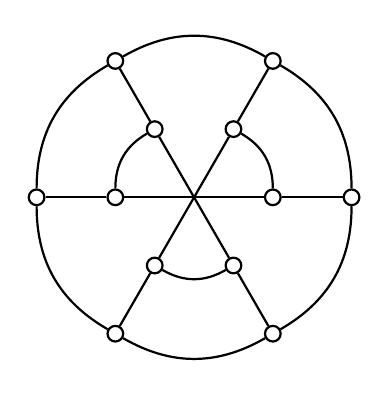
\begin{tikzpicture}
[lineDecorate/.style={-,thick},%
  nodeDecorate/.style={shape=circle,inner sep=2pt,draw,thick}]
%% nodes or vertices
\foreach \nodename/\x/\y in {
  0/2/0, 1/1/1.732, 2/-1/1.732, 3/-2/0, 4/-1/-1.732, 5/1/-1.732,
  6/1/0, 7/0.5/0.866, 8/-0.5/0.866, 9/-1/0, 10/-0.5/-0.866, 11/0.5/-0.866}
{
  \node (\nodename) at (\x,\y) [nodeDecorate] {};
}
%% edges or lines
\tikzstyle{EdgeStyle}=[-,thick]
\foreach \startnode/\endnode/\bend in {
  0/1/bend right, 0/5/bend left, 0/6/bend left=0, 1/2/bend right,
  1/7/bend left=0, 2/3/bend right, 2/8/bend left=0, 3/4/bend right,
  3/9/bend left=0, 4/5/bend right, 4/10/bend left=0, 5/11/bend left=0,
  6/7/bend right, 6/9/bend left=0, 7/10/bend left=0, 8/9/bend right,
  8/11/bend left=0, 10/11/bend right}
{
  \Edge[style=\bend](\startnode)(\endnode)
}
\end{tikzpicture}
}
\end{figure}

\end{document}
